\documentclass[12pt]{article}
\usepackage[utf8]{inputenc}
\usepackage{amsmath}
\usepackage{graphicx}
\usepackage{array}
\usepackage{geometry}
\geometry{margin=2.5cm}
\usepackage{titlesec}
\usepackage{float}
\titleformat{\section}{\centering\bfseries\uppercase}{\thesection}{1em}{}

\begin{document}

\section*{ {{ title }} }

\begin{minipage}[t]{0.48\textwidth}
\begin{tabular}{|l|c|}
\hline
Base (b) & {{ base }} m \\
Altura (h) & {{ altura }} m \\
Recubrimiento (r) & {{ recubrimiento }} m \\
Estribo (\ensuremath{\phi_e}) & {{ diam_estribo }} m \\
Varilla principal (\ensuremath{\phi_s}) & {{ diam_varilla }} m \\
f'c & {{ fc }} MPa \\
fy & {{ fy }} MPa \\
\hline
\end{tabular}
\end{minipage}
\hfill
\begin{minipage}[t]{0.48\textwidth}
\begin{figure}[H]
\centering
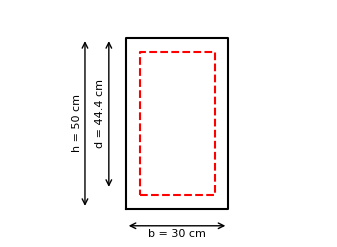
\includegraphics[height=5cm]{figures/section.png}
\end{figure}
\end{minipage}

\vspace{0.5cm}

\section*{Peralte: d (ART.PERALTE)}

\[
{{ formula_peralte }}
\]

Valor calculado: \( d = {{ d }}\,\text{m} \)

\begin{figure}[H]
\centering
\includegraphics[width=0.5\textwidth]{figures/peralte.png}
\end{figure}

\vspace{0.5cm}

\section*{Coeficiente B1 (ART.B1)}

\[
{{ formula_b1 }}
\]

Valor calculado: \( \beta_1 = {{ b1 }} \)

\begin{figure}[H]
\centering
\includegraphics[width=0.5\textwidth]{figures/b1.png}
\end{figure}

\vspace{0.5cm}

\section*{Pbal (ART.PBAL)}

\[
{{ formula_pbal }}
\]

Valor calculado: \( P_{bal} = {{ pbal }} \)

\begin{figure}[H]
\centering
\includegraphics[width=0.5\textwidth]{figures/pbal.png}
\end{figure}

\vspace{0.5cm}

\section*{\ensuremath{\rho_{bal}} (ART.RHOBAL)}

\[
{{ formula_rhobal }}
\]

Valor calculado: \( \rho_{bal} = {{ rhobal }} \)

\begin{figure}[H]
\centering
\includegraphics[width=0.5\textwidth]{figures/rhobal.png}
\end{figure}

\vspace{0.5cm}

\section*{Pmax (ART.PMAX)}

\[
{{ formula_pmax }}
\]

Valor calculado: \( P_{max} = {{ pmax }} \)

\begin{figure}[H]
\centering
\includegraphics[width=0.5\textwidth]{figures/pmax.png}
\end{figure}

\vspace{0.5cm}

\section*{As m\'in (ART.ASMIN)}

\[
{{ formula_asmin }}
\]

Valor calculado: \( A_{s}^{\text{min}} = {{ as_min }} \)

\begin{figure}[H]
\centering
\includegraphics[width=0.5\textwidth]{figures/asmin.png}
\end{figure}

\vspace{0.5cm}

\section*{As m\'ax (ART.ASMAX)}

\[
{{ formula_asmax }}
\]

Valor calculado: \( A_{s}^{\text{max}} = {{ as_max }} \)

\begin{figure}[H]
\centering
\includegraphics[width=0.5\textwidth]{figures/asmax.png}
\end{figure}

\end{document}
